
% example for dissertation.sty
\documentclass[
  % Replace oneside by twoside if you are printing your thesis on both sides
  % of the paper, leave as is for single sided prints or for viewing on screen.
  oneside,
  %twoside,
  11pt, a4paper,
  footinclude=true,
  headinclude=true,
  cleardoublepage=empty
]{scrbook}

\usepackage{dissertation}
\usepackage{movie15}

\newcommand{\name}{Musikla}
\newcommand{\fullname}{Music and Keyboard Language}

% ----------------------------------------------------------------

% Title
\titleA{\name}
\titleB{\fullname} % (if any)
\subtitleA{DSL de criação de acompanhamentos e}
\subtitleB{e teclados músicais programáveis} % (if any)

% Author
\author{Pedro M. Silva}

% Supervisor(s)
\supervisor{José João Almeida}
%\cosupervisor{The cosupervisor of the thesis}

% University (uncomment if you need to change default values)
% \def\school{Escola de Engenharia}
% \def\department{Departamento de Inform\'{a}tica}
% \def\university{Universidade do Minho}
% \def\masterdegree{Computer Science}

% Date
\date{\myear} % change to text if date is not today

% Keywords
%\keywords{master thesis}

% Glossaries & Acronyms
%\makeglossaries  %  either use this ...
%\makeindex	   % ... or this

% Define Acronyms
%%!TEX root = ../template.tex
%%%%%%%%%%%%%%%%%%%%%%%%%%%%%%%%%%%%%%%%%%%%%%%%%%%%%%%%%%%%%%%%%%%%
%% glossary.tex
%% NOVA thesis document file
%%
%% Acronyms definition
%%%%%%%%%%%%%%%%%%%%%%%%%%%%%%%%%%%%%%%%%%%%%%%%%%%%%%%%%%%%%%%%%%%%
\newacronym{daw}{DAW}{Digital Audio Workstation}
\newacronym{dsl}{DSL}{Domain Specific Language}
\newacronym{pcm}{PCM}{Pulse-Code Modulation}
\newacronym{midi}{MIDI}{Music Instrument Digital Interface}
\newacronym{wav}{WAV}{Waveform Audio File Format}
\newacronym{vm}{VM}{Virtual Machine}
\newacronym{mml}{MML}{Music Macro Language}
\newacronym{peg}{PEG}{Parsing Expression Grammar}
\newacronym{cfg}{CFG}{Context Free Grammar}
\newacronym{io}{I/O}{Input/Output}
\newacronym{ast}{AST}{Abstract Syntax Tree}
\newacronym{jit}{JIT}{Just In Time}
\newacronym{aot}{AOT}{Ahead Of Time}
\newacronym{api}{API}{Aplication Public Interface}
\newacronym{svg}{SVG}{Scalable Vector Graphics}
\newacronym{html}{HTML}{HyperText Markup Language}
\newacronym{ide}{IDE}{Integrated Development Environment}

%\loadglsentries[\acronymtype]{example-glossaries-acronym.tex}
%\glsaddall

%\glsaddall[types={\acronymtype}]

\newacronym{daw}{DAW}{Digital Audio Workstation}
\newacronym{dsl}{DSL}{Domain Specific Language}
\newacronym{pcm}{PCM}{Pulse-Code Modulation}
\newacronym{midi}{MIDI}{Music Instrument Digital Interface}
\newacronym{wav}{WAV}{Waveform Audio File Format}
\newacronym{vm}{VM}{Virtual Machine}
\newacronym{mml}{MML}{Music Macro Language}
\newacronym{peg}{PEG}{Parsing Expression Grammar}
\newacronym{cfg}{CFG}{Context Free Grammar}
\newacronym{io}{I/O}{Input/Output}
\newacronym{ast}{AST}{Abstract Syntax Tree}

\ummetadata % add metadata to the document (author, publisher, ...)

\begin{document}
	% Cover page ---------------------------------------
	\umfrontcover	
	\umtitlepage
	
	% Add acknowledgements ----------------------------
	%\chapter*{Acknowledgements}
	%Write acknowledgements here


	% Add abstracts (en,pt) ---------------------------
	\chapter*{Abstract}
	The creation of music using synthesizers is a practice that boasts many decades of existence. With the proliferation of personal computers, digital synthesizers and Digital Audio Workstations rose in popularity as well.
	
	This project aims to use the digital audio production and manipulation technologies, and wrap them in a domain specific language that allows to easily describe music compositions, generate sounds dynamically, study properties of music theory or even create virtual keyboards that play sounds or execute actions and can be used to perform live multimedia shows.
	
	\cleardoublepage
	\chapter*{Resumo}
	A criação de música usando sintetizadores é uma prática que conta já com várias décadas de uso. Com a proliferação dos computadores pessoais, popularizaram-se também os sintetizadores digitais e as Digital Audio Workstations.
	
	Este projeto tem como objetivo utilizar as tecnologias de produção e manipualação de aúdio digital, e envolvê-las numa linguagem de domínio específico que permita facilmente descrever composições músicais, gerar sons dinâmicamente, estudar propriedades da própria teoria músical, ou até criar teclados virtuais que toquem sons ou executem ações e podem ser utilizados para realizar espetáculos multimédia ao vivo.
	

	% Summary Lists ------------------------------------
	\tableofcontents
	\listoffigures
	\listoftables
	%\lstlistoflistings
	%\listofabbreviations
	
	
	\pagenumbering{arabic}
	
	% CHAPTER - Introduction -------------------------
	\chapter{Introdução}
	
	% Context,\\ motivation,\\ main aims	(objectives) \\ research hypothesis, (optional) \\ paper organization!
    O objetivo deste trabalho é estudar e prototipar formas de criação de música com recurso a técnicas habitualmente usadas na criação de \textit{software}. Para além de permitir criar música através das notas introduzidas manualmente, a linguagem deve facilitar a geração de música de um modo mais dinâmico, com recurso a operações de combinação e transformação de notas, como concatenar e misturar música.
    
    O termo música neste contexto é usado num sentido mais amplo que apenas sons. O objetivo desta linguagem é permitir gerar vários \textit{outputs} através do mesmo código fonte, como pautas músicais, ABC, WAV, MIDI, entre outros.

    Uma das partes mais críticas relativas à pesquisa e desenvolvimento necessários para a realização desta linguagem é a componente temporal implícita em todos os aspetos da linguagem: deve ser possível de um modo intuítivo expressar as várias composições possíveis de notas sem ser necessário expressar os tempos manualmente, tais como notas sequênciais, notas em paralelo, acordes, pequenas pausas e grandes pausas, bem como sincronizar partes da música de modo simples.

	% CHAPTER - State of the Art ---------------------
	\chapter{Estado da Arte}
    Atualmente a produção de música é realizada utilizando programas com interfaces gráficas, geralmente denominados como \acrfull{daw}. A minha abordagem irá consistir em estudar formas de criar e tocar músicas ao vivo (e não só) através de uma \acrfull{dsl}, usando técnicas inspiradas nas linguagens de programação e no desenvolvimento de \textit{software}.

	\section{Trabalho Relacionado}
	Existem diversos tipos de linguagens usadas atualmente para produzir ou simplesmente descrever música. Algumas fazem uso do conceito de notas músicais, com recurso a algum sintetizador externo, para gerar os sons, enquanto outras funcionam com base na manipulação direta de ondes de som digitais para criar música. Algumas suportam apenas a descrição estática da música, enquanto outras permitem formas dinâmicas tais como funções, variáveis, estruturas de controlo e repetição, ou até mesmo algorítmos aleatórios que permitem gerar músicas diferentes a cada execução.
	
	Iremos de seguida analisar algumas das soluções disponíveis atualmente, bem como comparar as funcionalidades que cada uma oferece ou não oferece em relação aos objetivos deste projeto.
	\subsection{Alda}
	O projeto \textbf{alda}\cite{alda} é uma linguagem de música textual desenvolvida em \textit{JAVA} focada na simplicidade: o seu maior ponto de atração é apelar tanto a programadores com pouca experiência musical, bem como a músicos com pouca experiência com programação.
    Apesar de ser anunciada como direcionada tanto a músicos como a programadores, a linguagem não suporta nenhum tipo de construções dinâmicas, como ciclos ou funções. Este tipo de funcionalidades, se necessário, requer o uso de uma linguagem de programação por cima, que poderia por exemplo, gerar o código \textit{alda} em \textit{runtime} através da manipulação de \textit{strings} antes de o executar. Isto significa que não é possível implementar composições interativas.
	
	\subsubsection{Exemplos}
	O exemplo seguinte demonstra um simples programa escrito em \textit{alda}, demonstrando: a seleção de um instrumento (\texttt{piano:}), a definição da oitava base (\texttt{o3}), um acorde com quatro notas (\texttt{c1/e/g/>c4}) em que a última se encontra uma oitava acima das outras.
\begin{lstlisting}[backgroundcolor=\color{transparent},caption={Exemplo da linguagem alda},captionpos=b,xleftmargin=.28\textwidth]
piano: o3 c1/e/g/>c4 < b a g | < g+1/b/>e
\end{lstlisting}
 É também possível verificar o uso de acidentais (identificados pelos símbolos \texttt{+} ou \texttt{-} a seguir a uma nota) bem como a diferenciação da duração de algumas notas (identificadas pelos números em frente às notas).
	\subsection{ABC Notation}
	A notação \textbf{ABC}\cite{abc-notation} é uma notação textual que permite descrever notação músical. É bastante completa, tendo formas de descrever notas, acordes, acidentais, uniões de notas, \textit{lyrics}, múltiplas vozes, entre outros.
	
	Para além das exaustividade de sintaxe que permite descrever quase todo o tipo de música, a popularidade da linguagem também significa que existem já inúmeros conversores de ficheiros ABC para os mais diversos formatos, desde ficheiros MIDI, pautas músicais, ou mesmo ficheiros WAV (gerados através do fornecimento de um ficheiro SoundFont, por exemplo).
	
	A complexidade da notação traz tanto vantagens como desvantages, no entanto: A sua ubiquidade significa que uma maior percentagem de utilizadores já se pode sentir à vontade com a sintaxe, o que não acontece com outras linguagens menos conhecidas. Mas por outro lado, conhecer ou implementar toda a especificação \cite{abc-notation-standard} é um feito bastante difícil.
	
	No entanto, tal como a linguagem \textit{ALDA}, as músicas definidas são estáticas, pelo que não serve como uma linguagem de programação de músicas dinâmicas. Ainda assim, apesar de implementar toda a notação ser algo pouco prático, implementar um \textit{subset} da notação, contendo as construções mais usadas seria uma vantagem enorme que me permitiria aproveitar a familiaridade de muitos utilizadores com as partes mais comuns da sintaxe.
	
		\subsubsection{Exemplos}
	A sintaxe de um ficheiro \textit{ABC} é composta por duas partes: um cabeçalho onde são definidas as configurações da música atual, seguido pelo corpo da música. O cabeçalho é formado por uma várias linhas. Cada linha, em ABC chamada de campo, tem uma chave e um valor separados por dois pontos (\texttt{:}). A especificação da notação descreve bastantes campos possíves, mas os mais usados são: \textbf{X} (número de referência), \textbf{T} (título), \textbf{M} (compasso), \textbf{L} (unidade de duração de nota) e \textbf{K} (clave).
	
	\begin{lstlisting}[backgroundcolor=\color{transparent},caption={Exemplo da notação ABC},captionpos=b,xleftmargin=.1\textwidth]
	C, D, E, F,|G, A, B, C|D E F G|A B c d|e f g a|b c' d' e'|f' g' a' b'|]
	\end{lstlisting}
	
	No exemplo acima podemos ver uma escala completa das notas (sem acidentais). O chamado C médio é representado por um \textbf{c} minúsculo (a capitalização das letras muda o significado). Para subir uma oitava, podemos anotar as notas com um apóstrofo (\textbf{c'}). As oitavas subsequentes são anotadas por mais apóstrofos. De modo análogo, para baixar uma oitava, devemos usar primeiro a nota em maíuscula (\textbf{C}). As oitavas anteriores são identificadas por uma (ou mais) vírgula a seguir à nota com letra maíuscula (\textbf{C,}).
	
	
	\begin{lstlisting}[backgroundcolor=\color{transparent},caption={Exemplo da notação ABC},captionpos=b,xleftmargin=.24\textwidth]
	A/2 A/ A A2 __A _A =A ^A ^^A [CEGc] [C2G2] [CE][DF]
	\end{lstlisting}
	A duração das notas pode ser ajustada relativamente à unidade global definida no cabeçalho acrescentando um número (por exemplo \textbf{2}) ou fração \textbf{1/4} à nota. Os acidentais bemol, bequadro e sustenido podem ser adicionados acrescentando um \textbf{\_}, \textbf{=} e \textbf{\^} antes da nota, respetivamente. Acordes (notas tocadas ao mesmo tempo) podem ser definidas entre parênteses retos (\textbf{[} e \textbf{]}).
	
	A notação disponibiliza muitos mais exemplos de todas as funcionalidades aceites no seu website\cite{abc-notation-examples}.
	
	\subsection{Faust}
	A linguagem \textbf{Faust}\cite{faust} é uma linguagem de programação funcional com foco na sintetização de som e processamento de audio. Ao contrário das linguagens analisadas até agora, não trabalha com abstrações de notas e elementos músicais. Em vez disso, a linguagem trabalha diretamente com ondas sonoras (representadas como \textit{streams} de números) e através de expressões matemáticas, que de uma forma funcional permite assim manipular o som produzido.
	
	Um dos pontos fortes da linguagem é o facto da sua arquitetura ser construída de raiz para compilar o mesmo código fonte em várias linguagens. De facto, o projeto conta com várias dezenas de \textit{targets}, desde os mais óbvios (C, C++, Java, JavaScript) até alguns mais especializados (WebAssembly, LLVM Bitcode, instrumentos VST/VSTi). Também permite gerar aplicações \textit{standalone} para as bibliotecas de audio mais comuns\cite{faust-targets}.
	
		A linguagem vem embutida com uma biblioteca extremamente completa\cite{faust-libraries} que implementa, entre muitas outras, funções de matemática comuns, filtros audio, funcionalidades extremamente básicas de interfaces gráficas que permitem controlar em tempo real os valores do programa (como botões e \textit{sliders} entre outros).
	
	\subsubsection{Exemplos}
	A documentação do projeto conta com uma quantidade abundante de exemplos\cite{faust-examples} e com um tutorial para iniciantes à \cite{faust-quickstart}, do qual irei colocar aqui alguns pequenos pedaços de código que demonstram as capacidades fundamentais da linguagem.
	
    \begin{lstlisting}[caption={Geração de ruído aleatório com volume a metade}]
    import("stdfaust.lib");
    process = no.noise*0.5;
    \end{lstlisting}
    
	No primeiro exemplo, podemos ver a estrutura mais básica de um programa escrito em \textit{Faust}. Na primeira linha é importada a biblioteca \textit{standard} da linguagem. Na segunda linha podemos ver a \textit{keyword} \textbf{\texttt{process}}, que representa o \textit{input} e \textit{output} audio do nosso programa. Finalmente, em frente a essa \textit{keyword} podemos ver a expressão \texttt{no.noise*0.5}. Isto demonstra a utilização de construções da biblioteca \textit{standard}, como o gerador de ruído aleatório, bem como a utilização de operadores matemáticos usuais (neste caso a multiplicação) para manipular o audio, e diminuir o volume para metade.
	
    \begin{lstlisting}[caption={Geração de ruído aleatório com um filtro \textit{low-pass}}]
    import("stdfaust.lib");
    ctFreq = 500;
    q = 5;
    gain = 1;
    process = no.noise : fi.resonlp(ctFreq,q,gain);
    \end{lstlisting}
    Neste exemplo, estamos a usar o operador \texttt{:} para canalizar o \texttt{output} do gerador de ruído para um filtro \textit{low-pass}, que filtra todas as frequências acima de um valor de corte (a variável \texttt{ctFreq}). Aumentar esta variável resulta num som mais agudo, enquanto que ao diminui-la obtemos um som mais grave (pois o valor de corte é mais baixo, apenas os sons abaixo desse valor são passados).
    
    \begin{lstlisting}[caption={Geração de ruído aleatório com um filtro \textit{low-pass} controlada por uma interface}]
    import("stdfaust.lib");
    ctFreq = hslider("[0]cutoffFrequency",500,50,10000,0.01);
    q = hslider("[1]q",5,1,30,0.1);
    gain = hslider("[2]gain",1,0,1,0.01);
    t = button("[3]gate");
    process = no.noise : fi.resonlp(ctFreq,q,gain)*t;
    \end{lstlisting}
    Por fim podemos ver um exemplo igual ao anterior, mas em vez de ter os valores das variáveis estáticos (guardados nas variáveis \texttt{ctFreq}, \texttt{q} e \texttt{gain}), estes são controlados em tempo real pela interface definida pelas chamadas à função \texttt{hslider}. Foi também adicionada uma variável \texttt{t} com um botão \textit{"gate"}. Este produz o valor 0 (zero) quando está solto, e o valor 1 (um) quando está pressionado, valor que quando multiplicado pelo resto da expressão serve efetivamente como um \textit{on-off switch} para todo o sistema.
    
	\subsection{Sonic Pi}
	Possivelmente a linguagem que mais se aproxima do objetivo pretendido com este projeto, \textbf{Sonic Pi}\cite{sonic-pi} descreve-se como uma ferramenta de código para a criação e performance de música.
	
	A linguagem permite tocar notas (e também construções mais complexas a partir das mesmas, tais como acordes, arpégios e escalas, por exemplo). Para além disso permite tocar \textit{samples}, que são ficheiros \acrfull{wav}. A linguagem traz já consigo aproximadamente 164 \textit{samples} que podem ser livremente usadas, mas é também possível ao utilizador usar as suas.
	
	As músicas são compostas por \textbf{live loops}, que são grupos de sons. É possível ter vários \textit{live loops} a tocar simultâneamente. Dentro de cada \textit{live loop} o utilizador pode usar a função \texttt{play} para tocar notas, \texttt{sample} para reproduzir ficheiros \acrshort{wav}, ou \textit{sleep} para avançar o tempo. Para além disso a linguagem suporta, através da função \texttt{with\_fx} a reprodução de sons com efeitos (como \textit{reverb}, \textit{pan}, \textit{echo} entre muitos outros\cite{sonic-pi-fx}).
	
	Para além das capacidades músicais, a linguagem disponibiliza numa sintaxe similar a \textit{Ruby}, com construções de programação como ciclos, variáveis, estruturas de controlo, e até métodos para adicionar aleatoriedade à música tocada, permitindo escolher, por exemplo, qual a nota a tocar a seguir de uma lista de possibilidades.
	
	Apesar de tudas estas funcionalidades disponibilizadas, existem áreas onde o \textit{Sonic Pi} fica aquém dos objetivos pretendidos para este projeto. Por exemplo, apesar de permitir tanto receber como enviar eventos \acrshort{midi}, as suas capacidades de \acrfull{io} são bastante primitivas. Também não é fácil utilizar o teclado teclado do computador para tocar sons ou manipular o estado do programa. É possível fazê-lo, mas é bastante mais complicado do que seria de esperar (para além de exigir utilizar alguma linguagem de programação à parte).
	
	\subsubsection{Exemplos}
	\begin{lstlisting}[caption={Reproduzir um \textit{sample} com valores aleatórios}] 
    loop do
        sample :perc_bell, rate: (rrand 0.125, 1.5)
        sleep rrand(0, 2)
    end
    \end{lstlisting}
    Neste exemplo, podemos ver como a linguagem \textit{Sonic Pi} permite criar um \textit{loop}, onde podemos tocar sons (neste caso, um sample pré-definido chamado \texttt{perc\_bell}).
    
    É possível verificar também o uso da função \texttt{sleep} para gerir manualmente o avanço temporal da música (neste caso usando um valor escolhido aleatóriamente e entre 0 e 2 segundos).
    
    
    \begin{lstlisting}[caption={Reproduzir um notas de uma escala aleatórias, com efeito \textit{reverb}}] 
    with_fx :reverb, mix: 0.2 do
        loop do
            play scale(:Eb2, :major_pentatonic, num_octaves: 3).choose, release: 0.1, amp: rand
            sleep 0.1
        end
    end
    \end{lstlisting}
    Neste exemplo podemos observar a possibilidade do uso de efeitos, em particular do efeito \texttt{reverb}, para manipular o som gerado pelo programa. Dentro do \textit{loop}, é tocada uma nota a cada 100 milisegundos. A função \texttt{scale} gera uma lista com as notas da escala pedida, e a função \texttt{choose} escolhe aleatóriamente uma dessas notas para tocar.
    
	\section{Gramáticas}
	%% PEG vs CFG:
%%  - Em PEGs, o operador de escolha / é ordenado, i.e. é relevante a ordem por que as várias alternativas são colocadas.
%%    Numa CFG, o operador de escolha não é ordenado, o que pode resultar em gramáticas ambíguas, onde o mesmo input pode resultar em diferentes parse trees.
%% https://stackoverflow.com/questions/34976533/some-information-about-peg-needed
%% https://en.wikipedia.org/wiki/Parsing_expression_grammar
%% https://compilers.iecc.com/comparch/article/05-09-114


Para além dos aspetos técnicos da geração e reprodução de música já abordados neste relatório, existe também um componente fulcral relativo à análise e interpretação da linguagem que irá controlar a geração dos sons. Uma das primeiras decisões a ser tomada diz respeito à escolha do \textit{parser}, e possivelmente, do tipo de gramática que irá servir de base para a geração do mesmo.

Tradicionalmente, as gramáticas mais populares no campo de processamento de texto tendem a ser \acrfull{cfg}, que são usadas como \textit{input} nos geradores de \textit{parser} mais populares (Bison/YACC, ANTLR). Existem no entanto alternativas, algumas até mais recentes, como as \acrfull{peg}, que trazem consigo diferenças que podem ser consideradas por alguns como vantagens ou desvantagens.

\subsection{Diferenças: \acrshort{cfg} vs \acrshort{peg}}

A diferença com maiores repercussões práticas entre as duas classes de gramáticas deve-se á semãntica atribuída ao operador de escolha, e a consequente \textbf{ambíguidade} (ou falta dela) na gramática. Nas gramáticas \acrshort{peg}, o operador é ordenado, o que significa que a ordem por que as alternativas aparecem é relevante durante o \textit{parsing} do \textit{input}. Isto contrasta com a semântica nas \acrshort{cfg}, onde a ordem das alternativas é irrelevante. Isto pode no entanto levar a ambíguidades, onde o mesmo \textit{input}, descrito pela mesma gramática, pode resultar em duas árvores de \textit{parsing} diferentes, se satisfizesse mais do que um dos ramos do operador de escolha. Isto é, as \acrshort{cfg} podem por essa razão ser ambíguas.

Tomemos como exemplo o famoso problema do \textit{dangling else}\cite{dangling-else} descrito nas duas classe de gramáticas:
\begin{center}
\begin{tabular}{c}
\begin{lstlisting}[backgroundcolor=\color{transparent}]
 if (a) if (b) f1(); else f2();
\end{lstlisting}
\end{tabular}
\end{center}

\begin{lstlisting}[caption=Gramática,captionpos=t]
 statement = ...
    | conditional_statement
 
 conditional_statement = ...
    | IF ( expression ) statement ELSE statement
    | IF ( expression ) statement
\end{lstlisting}

No caso de uma \acrshort{cfg}, sabendo que o operador de escolha \texttt{|} é comutativo, o seguinte \textit{input} será ambíguo, podendo resultar num \textit{if-else} dentro do \textit{if} ou num \textit{if} dentro de um \textit{if-else}.

Mas no caso de uma \acrshort{peg}, o resultado é claro: um \textit{if-else} dentro de um \textit{if}. Quando a primeira regra do condicional chega ao \texttt{statement}, este vai por sua vez chamar o não terminal \texttt{conditional\_statement}, que por sua vez irá consumir o \textit{input} até ao fim. Deste modo, quando a execução voltar ao primeiro \texttt{conditional\_statement}, esta irá falhar por não conseguir ler o \textit{else} (uma vez que já consumimos todo o texto de entrada). Irá depois irá usar a segunda alternativa, dando então o resultado previso.

Com este exemplo de \textit{backtracking} podemos também verificar um problema aparente nas gramáticas \acrshort{peg}. Falhando a primeira alternativa na produção \texttt{conditional\_statement}, a segunda irá ser testada. Mas é evidente, olhando para a gramática que a segunda alternativa é exatamente igual à parte inicial da primeira alternativa (que neste caso também corresponde á parte que teve sucesso). Em vez de voltar a testar as regras de uma forma \textit{naive}, as \acrlong{peg} guardam antes em \textit{cache} os resultados de testes anteriores, permitindo assim uma pesquisa em tempo linear relativamente ao tamanho do \textit{input}, à custa de uma maior utilização de memória.

%% TODO Talk about composition and why PEG grammars can do it better than CFG

\subsection{Resumo}
Em resumo, as três principais diferenças entre as tradicionais \acrfull{cfg} e as mais recentes \acrfull{peg} são:

\textbf{Ambiguidade}. O operador de escolha ser comutativo nas \acrshort{cfg} resulta em gramáticas que podem ser ambíguas para o mesmo \textit{input}. As \acrshort{peg} são determínisticas, mas exigem mais cuidado na ordem das produções, uma vez que tal afeta a semântica da gramática.

\textbf{Memoization} Para evitar \textit{backtracking} exponêncial, as \acrshort{peg} utilizam \textit{memoization} que lhes permite guardar em \textit{cache} resultados parciais durante o processo de \textit{parsing}. Isto reduz o tempo dispendido, pois evita fazer o \textit{parse} do mesmo texto pela mesma regra duas vezes. Mas também aumenta o consumo de memória, pois os resultados parciais têm de ser guardados até a análise terminar por completo.

\textbf{Composição} As \acrlong{peg} também têm a vantagem de oferecerem uma maior facilidade de composição. Em qualquer parte da gramática é possível trocar um terminal por um não terminal. Isto é, é extremamente fácil construir gramáticas mais modulares e compô-las entre si.

    \section{SoundFonts}
    O formato \textit{SoundFont} foi originalmente desenvolvido nos anos 90 pela empresa E-mu Systems para ser usado inicialmente pelas placas de som \textit{Sound Blaster}. Ao longo dos anos o formato sofreu diversas alterações, encontrando-se atualemente na versão 2.04, lançada em 2005\cite{soundfont}. Atualmente existem diversos sintetizadores de software \textit{cross platform} e \textit{open source} capazes de converterem eventos \textit{MIDI} em som usando ficheiros \textit{SoundFont}, dispensando a necessidade de uma placa de som compatível com o formato. Alguns destes projetos são TiMidity\verb|++|\cite{timidity}, WildMIDI\cite{wild-midi} e FluidSynth\cite{fluidsynth}.
    
    Para além do formato original, existem também alternativas mais recentes que disponibilizam mais funcionalidades na sua especificação, como os ficheiros \textbf{SFZ} ou \textbf{NKI}. Estas alternativas trazem consigo vantagens e desvantagens, mas independentemente dos seus méritos, até agora nenhuma atingiu a popularidade dos ficheiros \textit{SoundFont}, o que significa também menos bibliotecas e menos aplicações para trabalhar com elas.

    Um ficheiro de SoundFont é constítuido por um ou mais bancos (\textit{banks}) (até um máximo de 128). Cada banco pode por sua vez ter até 128 \textit{presets} (por vezes também chamados instrumentos ou programas).

    Usando a sintaxe de declaração de tipos do \textit{Python} (que irá ser usada mais vezes neste projeto), podemos declarar um \textit{SoundFont}, de uma forma bastante genérica e omitindo detalhes não essenciais, como sendo modelado pelos seguintes tipos:
    \newpage
    \begin{lstlisting}[caption=Sistema de Tipos de um ficheiro SoundFont,language=Python]
     # Cada preset e identificado por um par: (bank, preset number)
     SoundFont = Dict[ Tuple[ int, int ], Preset ]
     
     # Cada instrumento e identificado por um inteiro entre 0 e 127
     Preset = Dict[ int, Instrument ]
     
     # Finalmente, cada sample e identificada pelo indice de nota (que iremos abordar mais a frente em detalhe, no capitulo sobre sintetizadores)
     Instrument = Dict[ int, Sample ]
     
     # Aqui nao se encontram detalhados os tipos Wave nem SampleOptions.
     Sample = Tuple[ Wave, SampleOptions ]
    \end{lstlisting}


	\section{Sintetizadores}
	A biblioteca FluidSynth é um \textit{software} sintetizador de aúdio em tempo real que transforma dados MIDI em sons, que podem ser gravados em disco ou encaminhados diretamente para um \textit{output} de aúdio. Os sons são gerados com recurso a SoundFonts\cite{soundfont} (ficheiros com a extensão \texttt{.sf2}) que mapeiam cada nota para a gravação de um instrumento a tocar essa nota.

Os \textit{bindings} da biblioteca para Python foram baseados no código \textit{open source} do projeto \textbf{pyfluidsynth}\cite{pyfluidsynth}, jutamente com algumas definições CPython extra para permitir usar funções que não tivessem \textit{bindings} já criados.

\subsection{Inicialização}
Para utilizar a biblioteca FluidSynth, existem três objetos principais que devem ser criados: Settings (\texttt{fluid\_settings\_t*}), Synth (\texttt{fluid\_synth\_t*}) e AudioDriver (\texttt{fluid\_audio\_driver\_t*}).

O objeto \textbf{Settings}\cite{fluidsynth_settings} é implementado com recurso a um dicionário. Para cada chave (por exemplo, \texttt{``audio.driver''}) é possível associar um valor do tipo inteiro (\texttt{int}), \textit{string} (\texttt{str}) ou \textit{double} (\texttt{num}). Alguns valores podem ser também booleanos (\texttt{bool}), no entanto eles são armazenados como inteiros com os valores aceites sendo apenas 0 e 1.

O objeto \textbf{Synth} é utilizado para controlar o sintetizador e produzir os sons. Para isso é possível enviar as mensagens MIDI tais como \texttt{NoteOn}, \texttt{NoteOff}, \texttt{ProgramChange}, entre outros.

O terceiro objeto \textbf{AudioDriver} encaminha automaticamente os sons para algum \textit{audio output}, seja ele colunas no computador ou um ficheiro em disco. Os seguintes \textit{outputs} são suportados pela biblioteca:

\begin{adjustwidth}{20pt}{20pt}
\begin{description}
    \item[Linux:] jack, alsa, oss, PulseAudio, portaudio, sdl2, file
    \item[Windows:] jack, PulseAudio, dsound, portaudio, sdl2, file
    \item[Max OS:] jack, PulseAudio, coreaudio, portaudio, sndman, sdl2, file
    \item[Android:] opensles, oboe, file
\end{description}
\end{adjustwidth}

\subsection{Utilização}
Com os objetos necessários inicializados, é necessário ainda especificar qual (ou quais) a(s) \textit{SoundFont(s)} a utilizar. Para isso podemos chamar o método \texttt{Synth.LoadSoundFont} que recebe dois argumentos: uma \textit{string} com o caminho em disco do ficheiro \textit{SoundFont} a carregar, seguido dum booleano que indica se os \textit{presets} devem ser atualizados para os da nova \textit{SoundFont} (isto é, atribuir os instrumentos da \textit{SoundFont} aos canais automaticamente).

A função \texttt{Synth.NoteOn} recebe três argumentos: um inteiro a representar o canal, outro inteiro entre 0 e 127 a representar a nota, e finalmente outro inteiro também entre 0 e 127 a representar a velocidade da nota.

O canal (\textbf{channel}) representa qual o instrumento que vai reproduzir a nota em questão. Cada canal está atríbuido a um programa da SoundFont, e é possível a qualquer momento mudar o programa atribuido a qualquer canal através do método \texttt{Synth.ProgramChange}. Caso se tenha carregado mais do que uma \textit{SoundFont}, é possível usar o método \texttt{Synth.ProgramSelect}, que permite especificar o \texttt{id} da \textit{SoundFont} e do banco do instrumento a atribuir.

A chave (\textbf{key}) representa a nota a tocar. Sendo este valor um inteiro entre 0 e 127, é necessário saber como mapear as tradicionais notas músicais neste valor. Para isso, basta colocarmos as \textit{pich classes} e os seus respetivos acidentais \textit{sharp} numa lista ordenada (\verb|C, C#, D, D#, E, F, F#, G, G#, A, A#, B|) e associar a eles os inteiros entre 0 e 11 (inclusive). Depois apenas temos de somar a esse número a multiplicação da oitava da nota (a começar em 0) por 12. Podemos deste modo calcular, por exemplo, que a \textit{key} do C central (C4) é igual a 48 ($0 + 4 * 12$). Assim, podemos generalizar que para uma oitava $O$ e para um tom de nota $N$, obtemos a chave aplicando a fórmula:
$$N + O * 12$$

A velocidade (\textbf{velocity}) é também um valor entre 0 e 127. Relacionando a velocidade com um piano físico, esta representa a força (ou velocidade) com que a tecla foi premida. Velocidades maiores geram sons mais altos, enquanto que velocidades mais baixas geram sons mais baixos, permitindo assim ao músico dar ou tirar enfase a uma nota relativamente às restantes. De notar que um valor igual a zero é o equivalente a invocar o método \texttt{Synth.NoteOff}.

A método \texttt{Synth.NoteOff}, por sua vez, recebe apenas dois argumentos (canal e chave), e deve ser chamada passsado algum tempo para terminar a nota. Podemos deste modo construir a analogia óbvia que o método \texttt{NoteOn} corresponde a uma tecla de piano ser premida, e \texttt{NoteOff} corresponde a essa tecla ser libertada.


	% CHAPTER - Problem and Challenges ---------------
	\chapter{O problema e os seus desafios}
    Desenhar esta \acrfull{dsl} trás consigo os problemas comuns ao desenho de linguagens de programação, bem como desafios novos e únicos relativos ao domínio músical. Alguns desses desafios foram já bastante estudado pela míriade de linguagens de programação, tanto indústriais como académicas, que já foram desenvolvidas, pelo que não serão o foco principal deste projeto. Pelo contrário, neste projeto serão focados com mais detalhe os desafios resultantes da integração da componente músical na linguagem.
    
    O primeiro desses desafios é a introdução de um novo tipo de dados primitivo não existente na maioria das outras linguagens: \textbf{Música}. Este tipo de dados trás consigo a necessidade implícita de gerir o conceito de \textbf{tempo} na linguagem, tanto na geração de música \textit{realtime} como \textit{offline} (em que o tempo a que a música está a ser gerada pode ser mais rápido ou mais lento do que o tempo real). Este conceito de tempo também acaba por escapar para o campo da gramática e da sintaxe da linguagem, necessitando de uma forma de descrição do mesmo que seja flexível, mas não demasiado verbosa ou díficil de ler.
    
    Ainda relacionado com o tipo de dados \textit{Música}, também é importante pensar em como o representar, e os casos que deve cobrir. Para este fim, acho que é importante a linguagem permitir gerar sons \textbf{potêncialmente infinitos}. Esta funcionalidade não é tão útil no campo da geração de música \textit{offline}, mas é extremamente útil quando a música está a ser gerada em tempo real, e possivelmente a ser controlada por um utilizador através do teclado, permitindo começar a tocar música gerada proceduralmente, e deixá-la tocar durante o tempo que for necessário. Como tal é necessário pensar em como a implementação de todo o código depende deste ponto.

	\section{Solução Proposta}
	A linguagem irá ser desenvolvida em \textit{Python}. A linguagem irá ser extensível, permitindo ao utilizador definir objetos ou funções em \textit{Python} e expô-los para dentro da linguagem, dando assim acesso à grande quantidade de módulos já existentes para os mais variados fins.
	
	Como exemplo da extensibilidade da linguagem, irá também ser desenvolvido por cima dela uma biblioteca de construção de teclados virtuais que permitem associar a eventos de teclas notas ou sequências músicais, ou mesmo instruções a serem executadas na própria linguagem.
	
	Para resolver o problema da representação do tempo, toda a linguagem irá ter noção implícita desse conceito, mesmo que apenas algumas construções o utilizem. Isto significa que durante toda a execução, haverá uma variável de \textbf{contexto} que será implicitamente passada para todas instruções e todas as chamadas de funções que, entre outras coisas, irá manter registo da passagem do tempo. Desta forma os construtores que precisarem do contexto, como por exemplo a emissão de notas músicais, podem aceder ao tempo atual bem como modificá-lo.
	
	A existência deste \textbf{contexto} implícito significa que as funções \textit{Python} não podem ser expostas diretamente para a linguagem, mas graças à expressividade do \textit{Python} é possível construit uma \textit{Foreign Function Interface} que seja incrivelmente simples de usar e que evite que o utilizador tenha de mapear as funções manualmente. Em vez disso, pode simplesmente marcá-las como sendo \textbf{context-free} (funções que não têm noção da existência do contexto implícito), e elas serão então tratadas de forma apropriada.
	
	O tipo de dados \textbf{Música} irá ser implementado sobre o conceito de iteradores (e mais especificamente geradores) fornecido pelo \textit{Python} para tornar a criação de música \textit{lazy}. No entanto, este paradigma deve ser completamente opaco para o utilizador da linguagem: a decisão de usar o modelo de execução normal, ou funções geradores deve ser tomado em segundo plano pelo motor de execução da linguagem, sempre que este for necessário. Isto é, ao contrário da maioria das linguagens que exigem para a utilização de geradores que o utilizador declare explicitamente que quer "emitir" um valor através de alguma \textit{keyword}, geralmente \texttt{yield}, na nossa linguagem sempre que alguma função produzir um valor do tipo de música que não seja consumido de alguma forma (atribuido a uma variável ou passado a uma função, por exemplo), esse valor músical é \textbf{implicitamente emitido} para o gerador, uma vez que esse caso será o mais comum. Para evitar que o valor seja emitido, é necessário \textbf{descartá-lo manualmente} onde for caso disso. Se por outro lado a função lidar apenas com valores não-músicais, a sua execução irá seguir o modelo tradicional (onde a função termina a sua execução antes de retornar o controlo ao local onde foi chamada).
    \newpage
	\subsection{Gramática da Linguagem}
	A gramática completa da linguagem pode ser vista em \ref{grammar}. MAs antes de abordarmos em mais detalhe como irá der desenhada a gramática da linguagem, podemos aborar dois pequenos exemplos que demonstram a geração de notas músicais.
\begin{lstlisting}[caption=Exemplo da sintaxe proposta da linguagem,language=PHP]
V70 L1 T120;

fun melody () {
    V120;
    
    r/4 ^g/4 ^g/4 ^g/4;
    ^f/2 e/8 ^d3/8; 
    ^c2;
}

fun accomp () {
    V50; sustainoff();

    ^Cm;
    BM; 
    AM;
}

# Create the notes from a melody with a piano and accompany it with a violin in parallel
$notes = :piano melody() | :violin accomp();

# Play the notes twice
play( $notes * 2 );
\end{lstlisting}

	O desenho da gramática da linguagem é composto aproximadamente por três partes, todas elas interligadas entre si.
	\begin{description}
	 \item[Instruções e Declarações] Similar a quase todas as linguagens de programação, esta parte cobre a declaração de funções, variáveis, operadores e expressões em geral.
	 \item[Acompanhamentos Músicais] Um tipo de expressões especial, que em vez de produzir números ou \textit{strings} literais, reconhece expressões músicais (notas, acordes, etc).
	 \item[Teclados Virtuais] Açúcar sintático para facilitar a declaração de teclados virtuais. Para a lém de alguns construtores próprios, faz uso das expressões gerais e de acompanhamentos músicais descritas acima.
	\end{description}

	\subsubsection{Instruções e Expressões}
	As instruções e expressões da gramática são baseadas nas linguagens como C e JavaScript. Chavetas são usadas para delenear blocos de código. As variáveis são prefixadas com um dólar (\texttt{\$}) para prevenir ambiguidades com notas musicais. Cada instrução é separada com um ponto e vírgula (\texttt{;}) a menos que sejam blocos de código que terminem com o fechar de chavetas. Os parâmetros de funções são separados por vírgulas, mas como as vírgulas também são usadas para indicar a descida de oitava nas notas, o ponto e vírgula (\texttt{;}) pode ser usado nesses casos para prevenir ambiguidades.
	
	Em termos de instruções suportadas, a linguagem irá ter as usuais:
    \begin{description}
     \item[Declaração de Funções] \verb|fun function_name ( $arg1, $arg2, <...> ) {  }|
     \item[Ciclos While] \verb|while <condition> {  }|
     \item[Ciclos For] \verb|for $var in <expr> {  }|
     \item[Condicionais If] \verb|if <condition> {  } else {  }|
     \item[Atribuições a Variáveis] \verb|$var = <expr>;|
     \item[Chamada de Funções] \verb|function_name( <arg1>, <arg2>, <...> );|
    \end{description}
    
	\subsubsection{Acompanhamentos Musicais}
	A gramática de expressões ou acompanhamentos músicais tem como base fundamental os seguintes blocos: notas, pausas e modificadores. As notas são identificadas pelas letras A até G, seguindo a notação de \textit{Helmholtz}\cite{helmholtz-pitch-notation} para denotar as respetivas oitavas. Podem também ser seguidas de um número ou de uma fração, indicando a duração da nota.


\begin{center}
\begin{tabular}{c}
\textit{Exemplos de notas} \\
\begin{lstlisting}[backgroundcolor=\color{transparent}]
C,, C, C c c' c'' c''' c'/4 A1/4 B2
\end{lstlisting}
\end{tabular}
\end{center}

As notas podem depois ser compostas \textbf{sequencialmente} (como demonstrado em cima, em que cada nota avança o tempo pelo valor da sua duração) ou em \textbf{paralelo} (separados por uma barra vertical \texttt{|}, criando uma bifurcação do contexto em dois, que irão correr em paralelo). Devemos notar que o operador paralelo tem a menor precedência de todos, pelo que não é necessário agrupar as notas com parênteses quando se usa. Isto é, as duas expressões seguintes são equivalentes.

\begin{center}
\begin{tabular}{c}
\begin{lstlisting}[backgroundcolor=\color{transparent}]
    A B C | D E F
( A B C ) | ( D E F )
\end{lstlisting}
\end{tabular}
\end{center}

É também possível agrupar estes blocos com recurso a parênteses. Os grupos herdam o contexto da expressão superior, mas as modificações ao seu contexto permanecem locais. Isto permite, por exemplo, modificar configurações para apenas um conjunto restrito de notas. No exemplo seguinte, a velocidade da nota \texttt{C} é 70, mas para o grupo de notas \texttt{A B} a velocidade é 127.

\begin{center}
\begin{tabular}{c}
\begin{lstlisting}[backgroundcolor=\color{transparent}]
 v70 (v127 A B) C
\end{lstlisting}
\end{tabular}
\end{center}

Os modificadores disponíveis são:
\begin{description}
 \item[Velocity] A velocidade das notas, tendo o formato \texttt{[vV][0-9]+}.
 \item[Duração] A duração das notas, tendo o formato \texttt{[lL][0-9]+} ou \\ \texttt{[lL][0-9]+/[0-9]+}.
 \item[Tempo] O número de batidas por minuto (BPM) que definem a velocidade a que as notas são tocadas, tendo o formato \texttt{[tT][0-9]+}.
 \item[Assinatura de Tempo] Define a assinatura de tempo, que define o tipo de batida da música e o comprimento de uma barra na pauta musical. Tem o formato \texttt{[sS][0-9]+/[0-9]}.
\end{description}

É também poossível definir qual o instrumento a ser utilizado para as notas. Todas as notas pertencentes ao mesmo contexto depois do modificador utilizarão esse instrumento.

\begin{center}
\begin{tabular}{c}
\begin{lstlisting}[backgroundcolor=\color{transparent}]
 (:cello A F | :violin A D)
\end{lstlisting}
\end{tabular}
\end{center}

Para além destas funcionalidades, também existe algum açúcar sintático para algumas das tarefas mais comuns na construção de acompanhamentos, como tocar acordes ou repetir padrões.

\begin{center}
\begin{tabular}{c}
\begin{lstlisting}[backgroundcolor=\color{transparent}]
( [BG]*2 [B2G2] )*3
\end{lstlisting}
\end{tabular}
\end{center}
    
    \subsubsection{Teclados Virtuais}
    Para além de permitir declarar acompanhamentos músicais para serem tocados automaticamente, a linguagem permite declarar teclados virtuais. Associados às teclas do teclado podem estar notas, acordes, melodias, ou qualquer outro tipo de expressão suportado pela linguagem.
    
    
    \begin{lstlisting}[caption=Exemplo da sintaxe de teclados virtuais,language=PHP]
# Now an example of the keyboard. We can declare variables to hold state
$octave = 0;

$keyboard = @keyboard hold extend (v120) {
    # Keys can be declared to play notes
    a: C; s: D; d: E; f: F; g: G; h: A; j: B;
    # Or chords
    1: ^Cm; 2: BM; 3: AM;
        
    # Or any other expression, including code blocks that change the state
    z: { $octave = $octave - 1; };
    x: { $octave = $octave + 1; };
}

# The set_transform function allows changing all events before they are emitted by this keyboard
$keyboard::set_transform( $events => transpose( $events, octave = $octave ) );
    \end{lstlisting}

    Cada\label{modifiers} teclado aceita opcionalmente uma lista de modificadores, tais como:
    \begin{description}
     \item[hold] Começa a tocar quando a tecla é premida e acaba de tocar quando é solta
     \item[toggle] Começa a tocar quando a tecla é premida, e acaba de tocar quando ela é premida novamete
     \item[repeat] Quando a nota/acorde/música fornecida acaba de tocar, repete-a indefenidamente
     \item[extend] Em vez de tocar as notas de acordo com a sua duração, estende-as todas até a tecla ser levantada/premida novamente (quando usado em conjunto com \textbf{hold} ou \textbf{toggle}, respetivamente)
    \end{description}
    
    Também é possível passar uma expressão opcional entre parênteses que irá ser aplicada a todas as notas do teclado (no exemplo acima especificando um instrumento e o volume das notas com \texttt{(:violin v120)}), evitando assim ter de a repetir em vários sítios.
    
    Para além disso, será possível controlar muitos mais aspetos do teclado atribuindo-o a uma variável e chamando funções a partir daí, como por exemplo efetuar transformações nos eventos e notas emitidos, ou simular o carregar e soltar das teclas.

\begin{lstlisting}[caption=Exemplo da sintaxe proposta da linguagem,language=PHP]
# The set_transform function allows changing all events before they are emitted by this keyboard
$keyboard::set_transform( $events => transpose( $events, octave = $octave ) );
# It is possible to synchronize the keyboard with a grid to align the timings of key presses 
# and releases to said grid
$keyboard::set_grid( Grid::new( 1, 4 ) );
# We can also control the keys manually
$keyboard::start( "ctrl+z" );
$keyboard::stop_all();

\end{lstlisting}
    
    \subsection{Arquitetura do Sistema}
    O sistema irá ser composto por um interpretador de linguagem desenvolvido em Python, acompanhado por uma interface de linha de comandos que faça uso do interpretador.
     % TODO Float H position
	\begin{figure}[h]
	\begin{center}
		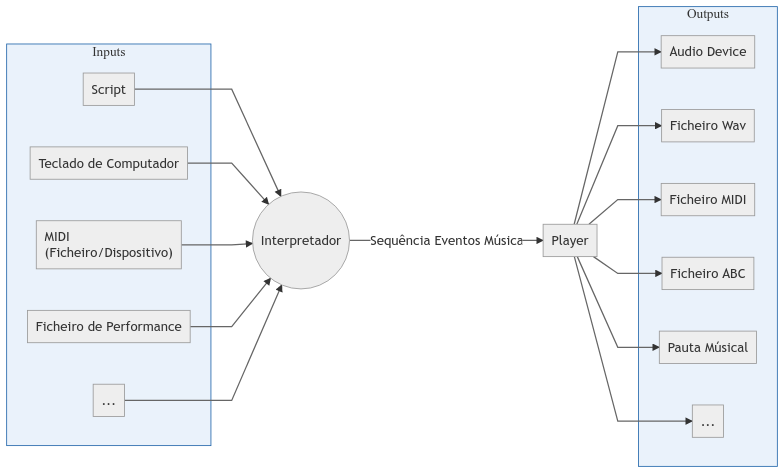
\includegraphics[width=0.87\textwidth]{img/diagram_architecture.png}
	\end{center}
	\caption{Arquitectura Geral do Projeto}
	\end{figure}
	
	O interpretador receberá um \textit{script} obrigatório como input. Esse input poderá depois determinar quais os \textit{inputs} (opcionais) que irá usar, como o teclado do computador, ficheiros ou teclados \acrshort{midi}, ficheiros de performance (gravações de reproduções anteriores consistindo nos eventos em que as teclas foram premidas).
	
	Os eventos gerados pelo \textit{script} e os restantes \textit{inputs} serão depois redirecionados para os diversos \textit{outputs}, que podem ser as colunas do dispositivo, ficheiros \acrshort{wav} ou \acrshort{midi}, ficheiros em formato PDF com a pauta músical, entre outros.
	
	Toda a linguagem irá ser desenvolvida com extensibilidade em mente nos seguintes pontos:
	\begin{description}
	 \item[Inputs] Permitir a criação de novos \textit{inputs}, como estar à espera de mensagens por um \textit{socket} ou de outros processos do computador.
	 \item[Eventos] A linguagem já disponibiliza uma variedade de eventos multimédia (como reproduzir notas, sons genéricos, ou mensagens para controlar dispositivos \acrshort{midi}). Mas o objetivo é que criar e emitir eventos customizados seja extremamente simples (e feito com uma só linha de código por evento, no mínimo). Obviamente, nem todos os eventos são suportados por todos os outputs (por exemplo, um ficheiro ABC não pode reproduzir um ficheiro \acrshort{wav}), mas neste caso os diversos \textit{outputs} irão simplesmente ignorar os eventos que não estejam preparados para lidar.
	 \item[Outputs] Para além dos \textit{outputs} embutidos, permitir criar novos, tanto para outros formatos músicais, mas também para outros fins como controlar luzes, vídeo e imagens através da linguagem (em conjunto com os eventos personalizados) e permitir assim executar espectáculos multimédia completos a partir da linguagem.
	 \item[Bibliotecas] Expôr funções, variáveis e objetos adicionais, bem como possivelmente acrescentar dinamicamente sintaxe à linguagem (através de macros).
	\end{description}

	
     % TODO Float H position
	\begin{figure}[h]
	\begin{center}
		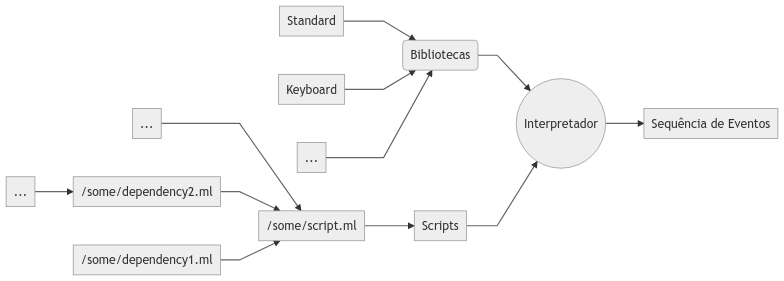
\includegraphics[width=0.95\textwidth]{img/diagram_virtualmachine.png}
	\end{center}
	\caption{Arquitectura do Interpretador}
	\end{figure}
    O facto de a linguagem ser desenvolvida em \textit{Python} significa que é extremamente prático extender a mesma devido a:
    \begin{itemize}
     \item Ubiquidade da linguagem Python tanto para programadores experiêntes como para iniciantes;
     \item Não ser necessário compilar o código para o executar;
     \item Sintaxe e expressividade da linguagem (apesar de vezes isso incorrer num custo de performance);
     \item Existência de \textit{bindings} para bibliotecas desenvolvidas em C/C++ (como \textit{numpy}), optimizadas para inúmeras tarefas que necessitem de maior \textit{performance}/menor latência, que mesmo assim expôem uma interface agradável de usar em \textit{Python};
    \end{itemize}

    \chapter{\name: Casos de Estudo}
    Neste capítulo iremos analisar possibilidades de uso da linguagem. Alguns desses exemplos são até já parcialmente ou totalmente funcionais quando executados no protótipo desenvolvido nesta fase inicial. Outros exemplos fazem uso de funcionalidades planeadas mas ainda não implementadas, e que serão devidamente identificados quando necessário.
    Nestes exemplos podem também ser usados pequenos excertos de músicas para demonstrar a utilização da linguagem, e a forma como esses excertos podiam ser representados com a nossa sintaxe.
    
    \section{Tocar Música}
    \begin{lstlisting}[caption=Exemplo da sintaxe para criação de música,language=PHP]
    # Title: Westworld Main Theme
    
    :piano = (1; S6/8 T70 L/8 V120 );
    :violin = :piano(41);
    
    $chorus = :piano (A*11 G F*12 | A,6 A,5 G, F,6*2)*3;

    $melody = :piano (r24   (:violin a3 c'3 d'3 e'9) r9 e'3 d'3 c'3 a9);

    play( $chorus | $melody );
    \end{lstlisting}
    
    % TODO Add back
    %\includemovie[text=\underline{Clicar para Reproduzir Aúdio}, attach=false]{}{}{../../code/SoundPlaygroundPy/examples/westworld.wav}
    
    Nas duas primeiras linhas deste exemplo podemos verifica a utilização de duas vozes (\texttt{:piano} e \texttt{:violin}). O piano ocupa a posição 1 da \textit{soundfont} utilizada, enquanto que o violino utiliza a posição 41. Ao declarar o piano, podemos também definir um conjunto de configurações adicionais (como o compasso, a duração base das notas, e o volume com que são tocadas). Ao declarar o violino, podemos herdar as configurações de outro instrumento (neste caso o piano) e mudar apenas o necessário (a posição do instrumento).
    
    Depois podemos ver a utilização de variáveis (\texttt{\$chorus} e \texttt{melody}) para estruturar e guardar conjuntos de notas, neste caso.
    É possível ver também o quão conciso fica descrever padrões ou conjuntos de notas repetidas através do operador de repetição (\texttt{*}). O operador de paralelo (\texttt{|}) permite depois tocar notas em paralelo ao mesmo tempo.
    
    \section{Definir um teclado}
    
    No início do capítulo \textbf{3.1.1} podemos ver um pequeno excerto de música que é tocada autonomamente pela linguagem. Aqui poderemos ver como construir um teclado virtual personalizado para tocar essa música, bem como a sequência de teclas a premir para a reproduzir.
        
    \begin{lstlisting}[caption=Exemplo da sintaxe para criação de teclados,language=PHP]
    # Title: Soft to Be Strong
    # Artist: Marina
    V70 L1 T120;

    fun toggle_sustain ( ref $enabled ) {
        if $enabled { cc( 64; 0 ) } else { cc( 64; 127 ) };

        $enabled = not $enabled;
    };
    
    $sustained = true;
    
    @keyboard hold extend {
        a: ^Cm;   s: BM;    d: AM;    f: EM;   g: ^Fm;
    };
    
    @keyboard hold extend (V120) {
        1: ^c;    2: ^d;    3: e;     4: ^f;   5: ^g;
        6: b;     7: ^c';   8: ^d';   9: e';

        c: toggle_sustain( $sustained );
    };
    \end{lstlisting}
    % TODO Add back
    % \includemovie[text=\underline{Clicar para Reproduzir Aúdio}, attach=false]{}{}{../../code/SoundPlaygroundPy/examples/marina.wav}
    
    No início deste exemplo podemos ver a declaração de uma função \textbf{toggle\_sustain}, que recebe como parâmetro uma variável por referência. O que isto significa é que qualquer alteração ao valor da variável dentro desta função, reflete-se também na variável que for passada à função quando esta é chamada. 
    
    Lá dentro fazemos uso da função \texttt{cc} que permite controlar diversos controlos \acrshort{midi}. Neste caso, o controlo \textit{64} refere-se ao pedal de \textit{sustain} de um piano (que deixa as notas a tocar durante mais algum tempo mesmo depois da sua tecla ser levantada). O valor 0 (\textit{zero}) que lhe é passado significa desligar esse pedal, e o valor \textit{127} significa ligar esse pedal. No futuro, apesar de ser sempre possível recorrer a este tipo de funções de baixo nível, irão ser adicionadas à biblioteca \textit{standard} as funções mais comuns (como por exemplo, \texttt{sustainoff()} e \texttt{sustainon()}).
    
    Depois podemos ver a declaração de dois teclados virtuais (a linguagem permite mais do que um teclado ativo ao mesmo tempo). O primeiro mapeia a algumas teclas (\texttt{a, s, d, f e g}) o conjunto de acordes usados nesta música. Para além disso também define alguns modificares a serem usados por este teclado (cujo significado é discutido no capítulo \ref{modifiers}).
    
    O segundo teclado funciona de forma similar, atribuíndo às teclas de 1 a 9 notas individuais a serem tocadas. Neste teclado podemos também ver que notas músicais não são os únicos elementos que podem ser associados a teclas. Também é possível descrever expressões arbitrárias (como neste caso, a chamada da função \texttt{toggle\_sustain( \$sustained )} associada à tecla \textbf{c}).
    
    Outro ponto a notar sobre o segundo teclado é a declaração entre parênteses \texttt{(V120)} que permite modificar o volume das notas tocadas por este teclado (que se sobrepõe ao volume global \texttt{V70} indicado no início do código). Isto é uma forma simples de prefixar configurações a todas as notas do teclado, evitando ter de copiar essas configurações para todas as notas.
    
    \section{QWERTY Keyboard}
    A função \texttt{qwertyboard} é uma função planeada a ser incluída na biblioteca \textit{standard} da linguagem. Aqui temos um exemplo simplificado do que essa função irá ser.
    Neste exemplo podemos observar funcionalidades mais genéricas da linguagem. Muitas dessas funcionalidades (arrays, métodos de objetos, funções anónimas) ainda não se encontram implementadas na versão atual do protótipo, mas servem como exemplo para o que a linguagem irá no fim permitir.
    \begin{lstlisting}[caption=Exemplo da sintaxe proposta da linguagem,language=PHP]
    fun qwertyboard () {
        # Maps the lines on a keyboard to semitone offsets to List[ List[ str ] ]
        $lines = @[
            "qwertyuiop"::split(),
            "asdfghjkl"::split(),
            "zxcvbnm,."::split()
        ];
        
        $octave = 0;
        $semitone = 0;
        
        $keyboard = @keyboard hold extend {
            [ $c for $c, $i in $lines::[ 0 ] ]: transpose( c; $i );
            [ $c for $c, $i in $lines::[ 1 ] ]: transpose( C; $i ); 
            [ $c for $c, $i in $lines::[ 2 ] ]: transpose( C,; $i );
            
            up => { $octave = $octave + 1 };
            down => { $octave = $octave - 1 };
            right => { $semitone = $semitone + 1 };
            left => { $semitone = $semitone - 1 };
        };
        
        $keyboard::set_transform( $events => $events + interval( 
            semitone = $semitone, 
            octave = $octave 
        ) );
        
        return $keyboard;
    }
    \end{lstlisting}
    A primeira parte da função declara um \textit{array} com as três linhas de caracteres presentes num teclado \textit{QUERTY}. Isto permite-nos ao declarar as teclas no \textit{keyboard}, fazê-lo de forma dinâmica (ao invés de associar a cada tecla uma nota manualmente).
    
    Essa declaração, inspirada nas listas por compreensão do \textit{Python}, funciona através de uma construção similar a um ciclo \textit{for}. A variável \texttt{\$c} corresponde a cada item do \textit{array} (neste caso, casa tecla), a variável \texttt{\$i} (opcional) permite-nos obter o índice da letra atual no \textit{array}. A cada letra é associada a nota \texttt{C} transposta pelo índice da tecla.
    
    Para além disso também podemos ver a declaração de mais quatro teclas (correspondentes às quatro setas do teclado) que permitem desclocar as notas tocadas por oitavas completas ou por semitons. Para isso, estas teclas têm associadas uma expressão de bloco (identificada peloas chavetas \texttt{\{} e \texttt{\}}). Lá dentro é possível meter uma instrução (ou opcionalmente várias, separadas por pontos e vírgulas \textbf{;}). O valor da última expressão é o valor de retorno da expressão de bloco toda, pelo que é possível que uma tecla faça mais que uma coisa (altere o estado e no fim retorne ainda notas para serem tocadas, por exemplo).
    
    Finalmente vemos também um exemplo do método \texttt{set\_transform}, um dos vários métodos que o objeto \texttt{Keyboard} irá ter e que permitem modificar ainda mais o comportamento dos teclados, desde transformar as teclas, definir grelhas de alinhamento, gravar as teclas premidas ou reproduzir uma dessas gravações, entre muitos outros.
    
    Este método, que aceita uma função como argumento, permite transformar cada evento músical que o teclado emita. Neste caso, estamos a usá-lo em conjunto com as variáveis de estado que declaramos anteriormente, para a cada evento, somar-lhe um intervalo composto pelos semitons e oitavas definidos.
    
    
	\chapter{Desenvolvimento}
	O desenvolvimento do projeto pode ser dividido de grosso modo em três. Nessas três camadas são cobertos um grupo abrangente de aspetos tanto da área do processamento de linguagens e do desenvolvimento de \acrshort{dsl}'s, da teoria músical, e do processamento digital de audio. 
	
	Na camada da linguagem esteve mais proeminente a área de processamento de linguagens, por motivos óbvios. Mas nas decisões tomadas durante o desenvolvimento desta camada, estiveram sempre presentes também as necessidades específicas que a teoria músical (e a sua notação) impõeem numa linguagem de programação.
	
	Do mesmo modo, o interpretador faz claramente uso de tópicos do domínio do processamento de linguagens, mas é ainda mais fortemente influencidado pelas restrições  e requisitos impostos pela componente músical da linguagem. Esta influencia a forma e a semântica da execução dos vários operadores disponibilizados.
	
	A última camada, de desenvolvimento de uma biblioteca, composta pelos objetos e procedimentos que têm como objetivo facilitar a utilização da linguagem. Para isso foi necessário identificar os casos de utilização mais comuns e prioritários, de modo a guiar a construção destas interfaces para refletirem uma utilização real da aplicação.
	
	\section{Linguagem}
	A camada sintática da aplicação pode ser conceptualmente dividida em duas fases:
	\begin{description}
	 \item[Sintaxe] Esta fase caracteriza-se por delinear qual a sintaxe usada pela linguagem, bem como os construtores e operadores suportados;
	 \item[Parser] Nesta fase foi desenvolvido um \textit{parser} em \textit{Python}, responsável por converter o código fonte da linguagem numa \acrfull{ast};
	\end{description}
	
	No entanto, a realidade é que a abordagem seguida (não só nesta camada mas como em todo o projeto) foi mais iterativa, dividindo cada faze em porções semi-independentes e intercalando as várias porções das diversas fases. Esta abordagem tem a vantagem de permitir ir testando e experimentando com o projeto mais cedo do que seria possível com um modelo de desenvolvimento em cascata.
	\subsection{Sintaxe}
	A sintaxe la linguagem é bastante inspirada nas usualmente chamadas linguagens da família C, com recurso a parênteses curvos e chavetas para delínear os vários blocos da linguagem.
	
	\subsection{Parser}
	\section{Interpretador}
	\section{Biblioteca Standard}
	\subsection{Inputs \& Outputs}
	\subsection{Ficheiros de Som}
	\subsection{Teclados Músicais}
	\subsection{Grelhas}
	\subsection{Transformadores}
	\subsection{Editor Embutido}
	

	% CHAPTER - Conclusion/Future Work --------------
	\chapter{Conclusão}
	O desenvolvimento do projeto envolve vários aspetos, desde o desenho da sintaxe e da gramática correspondente, até à geração de sons a serem guardados em ficheiros ou reproduzidos imediatamente em dispositivos aúdio. Também engloba tanto aspetos mais genéricos da programação, como qual a melhor forma de implementar de forma opaca funções geradoras e funções assíncronas.
	
	Mas para além disso também abrange quais as ferramentas e as metodologias são mais adequadas para a utilização da linguagem. É necessário para isso estudar com exemplos reais, qual a melhor forma de produzir e desenvolver música em formato textual.
	
	No entanto, sendo a criação músical uma área tão ampla, é ínutil tentar sequer conseguir desenvolver uma ferramenta que cubra todos os cantos e sirva todas as necessidades dos seus utilizadores. É por isso que é importante apoiar o desenvolvimento do projeto nas vantagens que a linguage \textit{Python} fornece, quer a nível da sua facilidade de uso, popularidade, e fácil extensão sem necessidade de processos complicados de compilação.
	
	O projeto deve ser por isso desenvolvido com extensibilidade em mente, tendo como objetivo principal servir como uma fundação estável capaz de ligar as diversas ferramentas existentes, não só na área da música, mas permitir ligar a música a outras áreas.
    
	\bookmarksetup{startatroot} % Ends last part.
	\addtocontents{toc}{\bigskip} % Making the table of contents look good.
	%\cleardoublepage

	%- Bibliography (needs bibtex) -%
	\bibliography{dissertation}

	% Index of terms (needs  makeindex) -------------
	%\printindex
	
	
	% APPENDIX --------------------------------------
	\umappendix{Appendix}
	
	% Add appendix chapters
	\chapter{Appendix}
	\section{Gramática}
	\label{grammar}
	\begin{lstlisting}
main <- body EOF;

body <- statement ( ";" statement )* _ ";"? _
      / ""
      ;

// Statements
statement <- _ ( var_declaration / voice_declaration / function_declaration / for_loop_statement / while_loop_statement / if_statement / expression ) _;

var_declaration <- "$" namespaced _ "=" _ expression;

voice_declaration <- ":" identifier _ "=" _ voice_declaration_body;

voice_declaration_body <- integer
                        / "(" _ function_parameters _ ")"
                        / ":" identifier _ "(" _ function_parameters _ ")"
                        ;

function_declaration <- "fun" _ namespaced _ "(" _ arguments? _ ")" _ "{" body "}";

arguments <- single_argument ( _ ";" _ single_argument )*;

single_argument <- single_argument_expr / single_argument_ref / single_argument_eval;

single_argument_expr <- "expr" _ "$" identifier;

single_argument_ref <- "ref" _ "$" identifier;

single_argument_eval <- "$" identifier;

for_loop_statement <- "for" _ "$" namespaced _ "in" _ value_expression _ ".." _ value_expression _ "{" _ body? _ "}";

while_loop_statement <- "while" _ expression _ "{" _ body _ "}";

if_statement <- "if" _ expression _ "{" _ body _ "}" _ "else" _ "{" _ body _ "}"
              / "if" _ expression _ "{" _ body _ "}";

// BEGIN Keyboard
keyboard_declaration <- "@keyboard" (_ alphanumeric)* ( _ group )? _ "{" ( _ keyboard_shortcut _  ";" )* _ "}";

keyboard_shortcut <- alphanumeric (_"+"_ alphanumeric)* (_ alphanumeric)* _ ":" _ expression
                   / string_value (_ alphanumeric)* _ ":" _ expression
                   / "[" _ list_comprehension _ "]" (alphanumeric _)* _ ":" _ expression
                   / "[" _ value_expression _ "]" (alphanumeric _)* _ ":" _ expression
                   ;

list_comprehension <- expression "for" _ "$" _ namespaced _ "in" _ value_expression _ ".." _ value_expression
                    / expression "for" _ "$" _ namespaced _ "in" _ value_expression _ ".." _ value_expression _ "if" value_expression
                    ;
// END Keyboard


expression <- e music_expression;

music_expression <- sequence ( _ "|" _ sequence )*;

sequence <- value_expression ( _ value_expression)*;

group <- "(" _ expression _ ")";

block <- "{" _ body _ "}";

note <- note_accidental _ note_pitch ( _ chord_suffix )? ( _ note_value )?;

chord_suffix <- 'M' / 'm';

variable <- "$" namespaced;

function <- namespaced "(" _ function_parameters? _ ")";

function_parameters <- expression ( _ ";" _ expression )*;

chord <- "[" _ note ( _ note )* _ "]";

rest <- "r" ( _ note_value )?;

note_value
    <- "/" _ integer
     / integer _ "/" _ integer
     / integer
     ;

note_accidental <- "^" / "^^" / "__" / "_" / "";

note_pitch
    <- r"[cdefgab]" "'"*
     / r"[CDEFGAB]" ","*
     ;

modifier
    <- r"[tT]" _ integer
     / r"[vV]" _ integer
     / r"[lL]" _ note_value
     / r"[sS]" _ integer _ "/" _ integer
     / r"[sS]" _ integer
     / r"[oO]" _ integer
     ;

instrument_modifier <- ":" ( identifier / "?" ) _ sequence;

value_expression <- expression expr_binary_op expression
                  / expr_unary_op expression
                  / string_value 
                  / number_value 
                  / bool_value 
                  / none_value 
                  / variable 
                  / function 
                  / keyboard_declaration 
                  / group 
                  / block 
                  / chord 
                  / note 
                  / rest 
                  / modifier 
                  / instrument_modifier
                  ;

exp_binary_op <- "and" / "or" / ">=" / ">" / "==" / "!=" / "<=" / "<" / r"[+\-*/]";

expr_unary_op <- "not";

string_value <- double_string / single_string;

double_string <- "\"" double_string_char* "\"";

double_string_char 
    <- "\\\""
     / "\\\\"
     / r"[^\"]"
     ;

single_string <- "'" single_string_char* "'";

single_string_char
    <- "\\'"
     / "\\\\"
     / r"[^']"
     ;

number_value <- float / integer;

bool_value <- "true" / "false";

none_value <- "none";

float <- r"[0-9]+\.[0-9]+";

integer <- r"[0-9]+";

namespaced <- ( identifier "\\" )* identifier;

identifier <- r"[a-zA-Z][a-zA-Z0-9\_]*";

alphanumeric <- r"[a-zA-Z0-9\_]*";

_ <- r"[ \t\r\n]*";

e <- "";

comment <- _ r"#[^\n]*";
	\end{lstlisting}

	%Auxiliary results which are not main-stream; or

	%\chapter{Details of results}
	%Details of results whose length would compromise readability of main text; or

	%\chapter{Listings}
	%Specifications and Code Listings: should this be the case; or

	%\chapter{Tooling}
	%Tooling: Should this be the case.

	%Anyone using \Latex\ should consider having a look at \TUG,
	%the \tug{\TeX\ Users Group}


	% Back Cover -------------------------------------------
	\umbackcover{
	%NB: place here information about funding, FCT project, etc in which the work is framed. Leave empty otherwise.
	}


\end{document}
